\documentclass[12pt]{article}
\usepackage[utf8]{inputenc}
\usepackage{amsmath, amssymb, graphicx}
\usepackage{geometry}
\geometry{margin=1in}
\usepackage{hyperref}
\usepackage{booktabs}
\usepackage{xcolor}
\usepackage{listings}
\usepackage{tikz}
\usetikzlibrary{trees}

% Code block style
\definecolor{codebg}{gray}{0.95}
\lstset{
  basicstyle=\ttfamily\small,
  backgroundcolor=\color{codebg},
  frame=single,
  breaklines=true
}

\title{\textbf{Machine Learning Principles}\\[0.4cm]
Homework 3}
\author{Raj Shah \\ Section: 01:198:461:03 \\ Professor: Kim Diana}
\date{Sunday, Due: November 16}

\begin{document}
\maketitle

\vspace{1em}

\newpage\textbf{1. [Decision Tree]} You will build a decision tree to determine whether or not a child goes out to play.

\begin{center}
\begin{tabular}{c c c c c c}
\toprule
Day & Weather & Temperature & Humidity & Wind & Play \\
\midrule
1  & Sunny  & Hot  & High   & Weak   & No  \\
2  & Cloudy & Hot  & High   & Weak   & Yes \\
3  & Sunny  & Mild & Normal & Strong & Yes \\
4  & Cloudy & Mild & High   & Strong & Yes \\
5  & Rainy  & Mild & High   & Strong & No  \\
6  & Rainy  & Cool & Normal & Strong & No  \\
7  & Rainy  & Mild & High   & Weak   & Yes \\
8  & Sunny  & Hot  & High   & Strong & No  \\
9  & Cloudy & Hot  & Normal & Weak   & Yes \\
10 & Rainy  & Mild & High   & Strong & No  \\
\bottomrule
\end{tabular}
\end{center}

\subsection*{1.1
Calculate the information gain for each feature and select the feature with the highest information gain to serve as the root of the decision tree. Draw a root and split the ten training data points into some groups based on the value of the selected root feature.}

\[
k^* = \arg\max_k I(X_k; Y) = H(Y) - H(Y \mid X_k)
\]
\subsection*{ANSWER:}
First, let's count the Play outcomes from the given data:
\begin{itemize}
    \item Yes: 5 instances (days 2, 3, 4, 7, 9)
    \item No: 5 instances (days 1, 5, 6, 8, 10)
\end{itemize}

\subsubsection*{Calculate $H(Y)$ - Entropy of Play:}
\begin{align*}
H(Y) &= -\frac{5}{10}\log_2\left(\frac{5}{10}\right) - \frac{5}{10}\log_2\left(\frac{5}{10}\right) \\
&= -0.5 \times (-1) - 0.5 \times (-1) \\
&= 1.0
\end{align*}

\subsubsection*{Information Gain for Weather:}

\textbf{Sunny (days 1, 3, 8):}
\begin{itemize}
    \item Yes: 1, No: 2
    \item $H = -\frac{1}{3}\log_2\left(\frac{1}{3}\right) - \frac{2}{3}\log_2\left(\frac{2}{3}\right) = 0.918$
\end{itemize}

\textbf{Cloudy (days 2, 4, 9):}
\begin{itemize}
    \item Yes: 3, No: 0
    \item $H = 0$ (pure)
\end{itemize}

\textbf{Rainy (days 5, 6, 7, 10):}
\begin{itemize}
    \item Yes: 1, No: 3
    \item $H = -\frac{1}{4}\log_2\left(\frac{1}{4}\right) - \frac{3}{4}\log_2\left(\frac{3}{4}\right) = 0.811$
\end{itemize}

\begin{align*}
H(Y|\text{Weather}) &= \frac{3}{10}(0.918) + \frac{3}{10}(0) + \frac{4}{10}(0.811) \\
&= 0.275 + 0 + 0.324 = 0.599
\end{align*}

\begin{equation*}
\boxed{IG(\text{Weather}) = 1.0 - 0.599 = 0.401}
\end{equation*}

\subsubsection*{Information Gain for Temperature:}

\textbf{Hot (days 1, 2, 8, 9):}
\begin{itemize}
    \item Yes: 2, No: 2
    \item $H = 1.0$
\end{itemize}

\textbf{Mild (days 3, 4, 5, 7, 10):}
\begin{itemize}
    \item Yes: 2, No: 3
    \item $H = -\frac{2}{5}\log_2\left(\frac{2}{5}\right) - \frac{3}{5}\log_2\left(\frac{3}{5}\right) = 0.971$
\end{itemize}

\textbf{Cool (day 6):}
\begin{itemize}
    \item Yes: 0, No: 1
    \item $H = 0$
\end{itemize}

\begin{align*}
H(Y|\text{Temperature}) &= \frac{4}{10}(1.0) + \frac{5}{10}(0.971) + \frac{1}{10}(0) \\
&= 0.4 + 0.486 + 0 = 0.886
\end{align*}

\begin{equation*}
\boxed{IG(\text{Temperature}) = 1.0 - 0.886 = 0.114}
\end{equation*}

\subsubsection*{Information Gain for Humidity:}

\textbf{High (days 1, 2, 4, 5, 7, 8, 10):}
\begin{itemize}
    \item Yes: 3, No: 4
    \item $H = -\frac{3}{7}\log_2\left(\frac{3}{7}\right) - \frac{4}{7}\log_2\left(\frac{4}{7}\right) = 0.985$
\end{itemize}

\textbf{Normal (days 3, 6, 9):}
\begin{itemize}
    \item Yes: 2, No: 1
    \item $H = -\frac{2}{3}\log_2\left(\frac{2}{3}\right) - \frac{1}{3}\log_2\left(\frac{1}{3}\right) = 0.918$
\end{itemize}

\begin{align*}
H(Y|\text{Humidity}) &= \frac{7}{10}(0.985) + \frac{3}{10}(0.918) \\
&= 0.690 + 0.275 = 0.965
\end{align*}

\begin{equation*}
\boxed{IG(\text{Humidity}) = 1.0 - 0.965 = 0.035}
\end{equation*}

\subsubsection*{Information Gain for Wind:}

\textbf{Weak (days 1, 2, 7, 9):}
\begin{itemize}
    \item Yes: 3, No: 1
    \item $H = -\frac{3}{4}\log_2\left(\frac{3}{4}\right) - \frac{1}{4}\log_2\left(\frac{1}{4}\right) = 0.811$
\end{itemize}

\textbf{Strong (days 3, 4, 5, 6, 8, 10):}
\begin{itemize}
    \item Yes: 2, No: 4
    \item $H = -\frac{2}{6}\log_2\left(\frac{2}{6}\right) - \frac{4}{6}\log_2\left(\frac{4}{6}\right) = 0.918$
\end{itemize}

\begin{align*}
H(Y|\text{Wind}) &= \frac{4}{10}(0.811) + \frac{6}{10}(0.918) \\
&= 0.324 + 0.551 = 0.875
\end{align*}

\begin{equation*}
\boxed{IG(\text{Wind}) = 1.0 - 0.875 = 0.125}
\end{equation*}

\subsubsection*{Summary of Information Gains:}
\begin{center}
\begin{tabular}{lc}
\toprule
\textbf{Feature} & \textbf{Information Gain} \\
\midrule
Weather & \textbf{0.401} (HIGHEST) \\
Temperature & 0.114 \\
Wind & 0.125 \\
Humidity & 0.035 \\
\bottomrule
\end{tabular}
\end{center}

\textbf{Weather has the highest information gain, so it becomes the root node.}

\subsection*{1.2
Repeat the two procedures:
\begin{enumerate}
    \item selecting a feature, and
    \item splitting the data points
\end{enumerate}
until the leaf nodes of the tree achieve complete purity.}
\subsection*{ANSWER:}
\subsubsection*{Root: Weather}

\textbf{Branch 1: Weather = Cloudy}
\begin{itemize}
    \item All instances (days 2, 4, 9) have Play = Yes
    \item \textbf{Leaf node: Yes} (pure)
\end{itemize}

\textbf{Branch 2: Weather = Sunny (days 1, 3, 8)}
\begin{itemize}
    \item Yes: 1, No: 2
\end{itemize}

Calculate IG for remaining features:

\textit{Temperature:}
\begin{itemize}
    \item Hot (1, 8): No, No $\rightarrow$ $H = 0$
    \item Mild (3): Yes $\rightarrow$ $H = 0$
    \item $IG = 1.0 - 0 = 1.0$ (HIGHEST)
\end{itemize}

Split on Temperature:
\begin{itemize}
    \item If Temp = Hot: \textbf{Play = No}
    \item If Temp = Mild: \textbf{Play = Yes}
\end{itemize}

\textbf{Branch 3: Weather = Rainy (days 5, 6, 7, 10)}
\begin{itemize}
    \item Yes: 1, No: 3
\end{itemize}

Calculate IG for remaining features:

\textit{Wind:}
\begin{itemize}
    \item Weak (7): Yes $\rightarrow$ $H = 0$
    \item Strong (5, 6, 10): No, No, No $\rightarrow$ $H = 0$
    \item $IG = 1.0 - 0 = 1.0$ (HIGHEST)
\end{itemize}

Split on Wind:
\begin{itemize}
    \item If Wind = Weak: \textbf{Play = Yes}
    \item If Wind = Strong: \textbf{Play = No}
\end{itemize}

\subsubsection*{Complete Decision Tree Visualization:}

\begin{center}
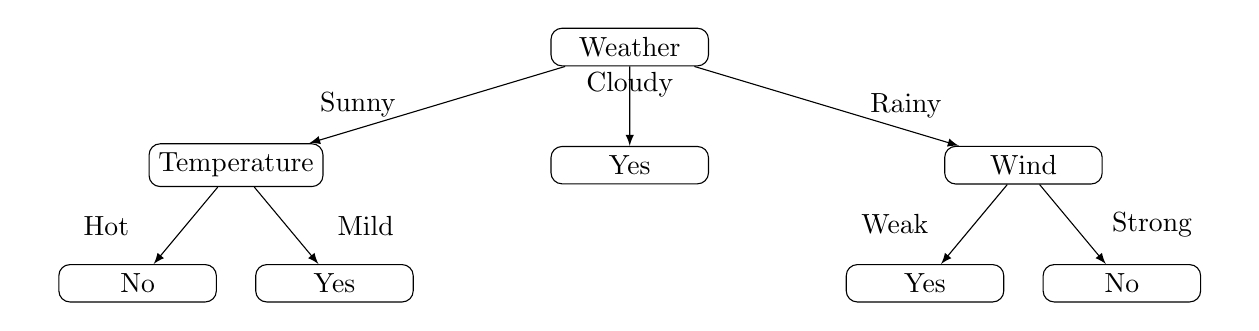
\begin{tikzpicture}[
  level 1/.style={sibling distance=50mm},
  level 2/.style={sibling distance=25mm},
  edge from parent/.style={draw, -latex},
  every node/.style={draw, rounded corners, align=center, minimum width=2cm}
]
\node {Weather}
  child {node {Temperature}
    child {node {No} edge from parent node[left, draw=none] {Hot}}
    child {node {Yes} edge from parent node[right, draw=none] {Mild}}
    edge from parent node[left, draw=none] {Sunny}
  }
  child {node {Yes}
    edge from parent node[above, draw=none] {Cloudy}
  }
  child {node {Wind}
    child {node {Yes} edge from parent node[left, draw=none] {Weak}}
    child {node {No} edge from parent node[right, draw=none] {Strong}}
    edge from parent node[right, draw=none] {Rainy}
  };
\end{tikzpicture}
\end{center}


\subsection*{1.3 [Extra Points: 10 points]}
Try pruning your tree. You need to find a subtree $T'$ minimizing the criterion $C(T')$ below. Based on the criterion computation, do you think we need to prune the tree found in 1.2? Please show how different range of $\lambda$'s results in the different decisions on tree pruning.

\[
C(T') = \sum_{\tau=1}^{T'} Q(\tau) + \lambda \cdot \lvert \text{num of leaves in } T' \rvert
\]

where
\[
Q(\tau) = \text{entropy of a leaf in } T' \; (\text{measure of impurity}).
\]

\vspace{1em}
\hrule
\vspace{1em}
\subsection*{ANSWER:}
For pruning analysis, we evaluate the cost-complexity criterion:

\begin{equation*}
C(T') = \sum_{i=1}^{|T'|} Q(\tau) + \lambda \cdot |\text{leaves in } T'|
\end{equation*}

Where $Q(\tau)$ is the entropy/impurity at leaf $\tau$.

\subsubsection*{Original Tree (T):}
\begin{itemize}
    \item 5 leaf nodes, all pure (entropy = 0)
    \item $C(T) = 0 + \lambda \cdot 5 = 5\lambda$
\end{itemize}

\subsubsection*{Potential Pruned Subtrees:}

\textbf{1. Prune Sunny $\rightarrow$ Temperature subtree:}
\begin{itemize}
    \item Replace with majority class (No, since 2 No vs 1 Yes)
    \item Impurity: $-\frac{2}{3}\log_2\left(\frac{2}{3}\right) - \frac{1}{3}\log_2\left(\frac{1}{3}\right) = 0.918$
    \item Weighted: $\frac{3}{10} \times 0.918 = 0.275$
    \item $C(T_1) = 0.275 + \lambda \cdot 4 = 0.275 + 4\lambda$
\end{itemize}

\textbf{2. Prune Rainy $\rightarrow$ Wind subtree:}
\begin{itemize}
    \item Replace with majority class (No, since 3 No vs 1 Yes)
    \item Impurity: $-\frac{3}{4}\log_2\left(\frac{3}{4}\right) - \frac{1}{4}\log_2\left(\frac{1}{4}\right) = 0.811$
    \item Weighted: $\frac{4}{10} \times 0.811 = 0.324$
    \item $C(T_2) = 0.324 + \lambda \cdot 4 = 0.324 + 4\lambda$
\end{itemize}

For pruning to be beneficial: $C(\text{pruned}) < C(\text{original})$

\begin{itemize}
    \item For Sunny subtree: $0.275 + 4\lambda < 5\lambda \Rightarrow 0.275 < \lambda$
    \item For Rainy subtree: $0.324 + 4\lambda < 5\lambda \Rightarrow 0.324 < \lambda$
\end{itemize}

\subsubsection*{Conclusion:}
\begin{itemize}
    \item If $\lambda > 0.324$, we should prune both subtrees
    \item If $0.275 < \lambda < 0.324$, prune only the Sunny subtree
    \item If $\lambda < 0.275$, don't prune
\end{itemize}

Different values of $\lambda$ (the complexity parameter) lead to different pruning decisions. Higher $\lambda$ values penalize tree complexity more, favoring simpler trees with fewer leaves even at the cost of some classification accuracy. Lower $\lambda$ values favor accuracy over simplicity, keeping more detailed splits.

\subsubsection*{Final Decision Tree Summary:}

The complete tree has:
\begin{itemize}
    \item \textbf{Root:} Weather (Information Gain = 0.401)
    \item \textbf{5 leaf nodes}, all achieving complete purity (100\% accuracy on training data)
    \item \textbf{Depth:} 2 levels
\end{itemize}

\textbf{Decision Rules:}
\begin{enumerate}
    \item If Cloudy $\rightarrow$ \textbf{Play}
    \item If Sunny \& Hot $\rightarrow$ \textbf{Don't Play}
    \item If Sunny \& Mild $\rightarrow$ \textbf{Play}
    \item If Rainy \& Weak Wind $\rightarrow$ \textbf{Play}
    \item If Rainy \& Strong Wind $\rightarrow$ \textbf{Don't Play}
\end{enumerate}

\vspace{1em}
\vspace{1em}


\newpage\textbf{2. [SVM]} In class, we learned a soft-margin SVM can be found by solving the dual problem below and SMO (Sequential Minimal Optimization) algorithm solves the dual problem. You will implement SMO based on a reference code and find a soft-margin SVM classifier to separate the two species of Iris: Iris-setosa and Iris-versicolor.

\[
\{\lambda_n^*\}_{n=1}^N = \arg\max_{\{\lambda_n\}_{n=1}^N}
\left(
- \frac{1}{2}
\sum_{n=1}^N
\sum_{m=1}^N
\lambda_n \lambda_m \, t_n t_m \, \kappa(x_n, x_m)
+
\sum_{n=1}^N \lambda_n
\right)
\]

subject to
\[
0 \le \lambda_n \le C,\quad n = 1, \dots, N,
\]
\[
\sum_{n=1}^N \lambda_n t_n = 0,
\]
where the kernel function is
\[
\kappa(x_n, x_m) = x_n^\top x_m.
\]

\subsection*{2.1
Read the paper SMO pages 6--11.\\[0.3em]
\url{https://www.microsoft.com/en-us/research/wp-content/uploads/1998/04/sequential-minimal-optimization.pdf}}
\subsection*{ANSWER:}
Platt’s SMO algorithm replaces the full quadratic program with a sequence of
two–variable subproblems. At each step, two multipliers $\lambda_1$ and $\lambda_2$
are updated analytically while satisfying:

\[
t_1 \lambda_1^{\text{new}} + t_2 \lambda_2^{\text{new}}
=
t_1 \lambda_1^{\text{old}} + t_2 \lambda_2^{\text{old}}.
\]

The error terms used in the update are:

\[
E_i = f(x_i) - t_i,
\qquad
f(x) = \sum_{j=1}^N \lambda_j t_j \kappa(x_j, x) + b.
\]

With the linear kernel $\kappa(x_i,x)=x_i^T x$, the decision function becomes:

\[
f(x)=w^T x+b,
\qquad
w=\sum_{j=1}^N \lambda_j t_j x_j.
\]

The unconstrained update for $\lambda_2$ is:

\[
\lambda_2^{\text{new, unc}} = 
\lambda_2^{\text{old}} + 
\frac{t_2(E_1 - E_2)}{\eta},
\qquad
\eta = 2 \kappa(x_1,x_2) - \kappa(x_1,x_1) - \kappa(x_2,x_2).
\]

\subsection*{2.2
Prove the bounds for clipping in equation (13) and (14) in the paper:
\[
\begin{cases}
y_1 \neq y_2: & L = \max(0, \lambda_2 - \lambda_1), \quad H = \min(C, C + \lambda_2 - \lambda_1)\\[0.3em]
y_1 = y_2:   & L = \max(0, \lambda_2 + \lambda_1 - C), \quad H = \min(C, \lambda_2 + \lambda_1)
\end{cases}
\]}
\subsection*{2.2
Refer to SMO implementation in code and write your SMO code \texttt{train2\_2.py} to solve the dual function with a linear kernel. Use \texttt{data.npz} for training.}
\subsection*{ANSWER:}
When updating only the two multipliers $\lambda_1$ and $\lambda_2$, the SMO algorithm
must satisfy the equality constraint of the dual problem:
\[
t_1 \lambda_1^{\text{new}} + t_2 \lambda_2^{\text{new}}
=
t_1 \lambda_1^{\text{old}} + t_2 \lambda_2^{\text{old}},
\]
where $t_i = y_i \in \{+1,-1\}$.

Solving for $\lambda_1^{\text{new}}$:
\[
\lambda_1^{\text{new}}
=
\lambda_1^{\text{old}}
+
t_1 t_2(\lambda_2^{\text{old}} - \lambda_2^{\text{new}}).
\]

We now derive the clipping bounds $L$ and $H$ for the two possible cases.

% -------------------------------------------------------------
\subsubsection*{Case 1: $y_1 \neq y_2$ (i.e., $t_1 t_2 = -1$)}
In this case,
\[
\lambda_1^{\text{new}}
=
\lambda_1^{\text{old}} + \lambda_2^{\text{new}} - \lambda_2^{\text{old}}.
\]

Let
\[
s = \lambda_1^{\text{old}} + \lambda_2^{\text{old}}.
\]
Then the equality constraint becomes
\[
\lambda_1^{\text{new}} + \lambda_2^{\text{new}} = s.
\]

Both multipliers must satisfy box constraints:
\[
0 \le \lambda_1^{\text{new}} \le C,
\qquad
0 \le \lambda_2^{\text{new}} \le C.
\]

Using $\lambda_1^{\text{new}} = s - \lambda_2^{\text{new}}$, the constraints imply
\[
0 \le s - \lambda_2^{\text{new}} \le C,
\qquad
0 \le \lambda_2^{\text{new}} \le C.
\]

From $s - \lambda_2^{\text{new}} \ge 0$:
\[
\lambda_2^{\text{new}} \le s.
\]

From $s - \lambda_2^{\text{new}} \le C$:
\[
\lambda_2^{\text{new}} \ge s - C.
\]

Thus the feasible interval is:
\[
L = \max(0,\, s - C) = \max(0,\, \lambda_2^{\text{old}} - \lambda_1^{\text{old}}),
\]
\[
H = \min(C,\, s) = \min(C,\, C + \lambda_2^{\text{old}} - \lambda_1^{\text{old}}).
\]

This reproduces Equation (13):
\[
\boxed{
L = \max(0,\, \lambda_2 - \lambda_1), \qquad
H = \min(C,\, C + \lambda_2 - \lambda_1)
}.
\]

% -------------------------------------------------------------
\subsubsection*{Case 2: $y_1 = y_2$ (i.e., $t_1 t_2 = +1$)}

In this case,
\[
\lambda_1^{\text{new}}
=
\lambda_1^{\text{old}}
+
\lambda_2^{\text{old}}
-
\lambda_2^{\text{new}}.
\]

Let
\[
s = \lambda_1^{\text{old}} - \lambda_2^{\text{old}}.
\]
Then
\[
\lambda_1^{\text{new}}
=
s + \lambda_2^{\text{new}}.
\]

Box constraints require:
\[
0 \le s + \lambda_2^{\text{new}} \le C,
\qquad
0 \le \lambda_2^{\text{new}} \le C.
\]

From $s + \lambda_2^{\text{new}} \ge 0$:
\[
\lambda_2^{\text{new}} \ge -s.
\]

From $s + \lambda_2^{\text{new}} \le C$:
\[
\lambda_2^{\text{new}} \le C - s.
\]

Thus:
\[
L = \max(0,\, -s) = \max(0,\, \lambda_2 + \lambda_1 - C),
\]
\[
H = \min(C,\, C - s) = \min(C,\, \lambda_2 + \lambda_1).
\]

This is Equation (14):
\[
\boxed{
L = \max(0,\, \lambda_2 + \lambda_1 - C), \qquad
H = \min(C,\, \lambda_2 + \lambda_1)
}.
\]
\subsection*{Important SMO Update Code (train2\_2.py)}

\begin{lstlisting}
# Compute Ei
f_i = np.sum(alphas * y * (X @ X[i])) + b
Ei  = f_i - y[i]

# Pick j != i
j = np.random.randint(0, m)
while j == i:
    j = np.random.randint(0, m)

f_j = np.sum(alphas * y * (X @ X[j])) + b
Ej  = f_j - y[j]

ai_old, aj_old = alphas[i], alphas[j]

# -----------------------------
# Clipping bounds (Eq. 13--14)
# -----------------------------
if y[i] != y[j]:
    L = max(0, aj_old - ai_old)
    H = min(C, C + aj_old - ai_old)
else:
    L = max(0, aj_old + ai_old - C)
    H = min(C, aj_old + ai_old)

if L == H:
    continue

# -----------------------------
# eta = 2 K(xi,xj) - K(xi,xi) - K(xj,xj)
# -----------------------------
eta = 2*np.dot(X[i], X[j]) \
      - np.dot(X[i], X[i]) \
      - np.dot(X[j], X[j])

if eta >= 0:
    continue

# -----------------------------
# Update alpha_j and clip
# -----------------------------
alphas[j] = aj_old - y[j] * (Ei - Ej) / eta
alphas[j] = np.clip(alphas[j], L, H)

if abs(alphas[j] - aj_old) < 1e-5:
    continue

# -----------------------------
# Update alpha_i
# -----------------------------
alphas[i] = ai_old + y[i]*y[j]*(aj_old - alphas[j])

# -----------------------------
# Update bias (b1, b2)
# -----------------------------
b1 = b - Ei \
     - y[i]*(alphas[i] - ai_old)*np.dot(X[i], X[i]) \
     - y[j]*(alphas[j] - aj_old)*np.dot(X[i], X[j])

b2 = b - Ej \
     - y[i]*(alphas[i] - ai_old)*np.dot(X[i], X[j]) \
     - y[j]*(alphas[j] - aj_old)*np.dot(X[j], X[j])

if 0 < alphas[i] < C:
    b = b1
elif 0 < alphas[j] < C:
    b = b2
else:
    b = (b1 + b2) / 2
\end{lstlisting}

% -------------------------------------------------------------
\subsubsection*{Conclusion}

In both cases, the equality constraint reduces the feasible region for $\lambda_2$
to a one-dimensional interval $[L,H]$.  
The SMO update computes the unconstrained value
\[
\lambda_2^{\text{new,unc}}
\]
and then clips it into this interval:
\[
\lambda_2^{\text{new}}
=
\text{clip}\left(
\lambda_2^{\text{new,unc}},\, L,\, H
\right).
\]

This completes the proof of the clipping bounds in Equations (13) and (14).

\newpage
\subsection*{2.3
\texttt{data.npz} contains Iris information including ``sepal length'' and ``sepal width''. In the data, Iris-setosa is coded as $+1$ and Iris-versicolor is coded as $-1$. Please run your SMO for $C = 1, 10, 100$ and plot the following for each $C$:
\begin{enumerate}
    \item decision boundary (black colored line),
    \item positive (red) margin,
    \item negative (blue) margin,
    \item positive training samples (red colored dots),
    \item negative training samples (blue colored dots).
\end{enumerate}}

\subsection*{ANSWER:}
Using the SMO implementation from 2.2, we train a linear SVM on the Iris dataset
(\texttt{data.npz}), where Iris-setosa is labeled $+1$ and Iris-versicolor is labeled $-1$.
For each $C \in \{1, 10, 100\}$, we plot:
\newpage
\subsection*{SVM Plot for $C = 1$}
\begin{figure}[h!]
\centering
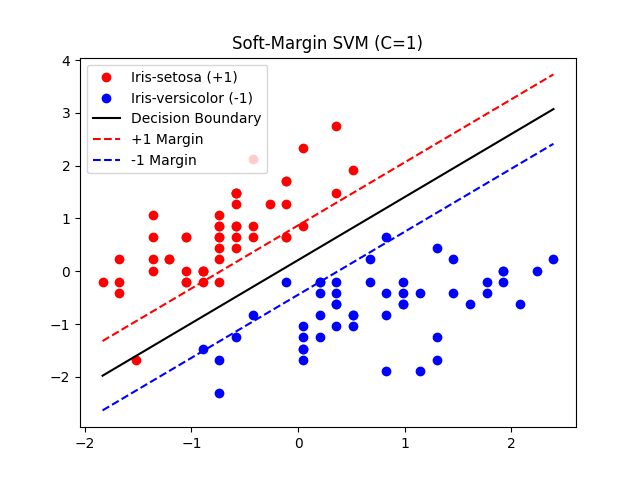
\includegraphics[width=0.65\textwidth]{svm_plot_C1.png}
\caption{Soft-margin SVM with $C=1$.}
\end{figure}
\newpage
\subsection*{SVM Plot for $C = 10$}
\begin{figure}[h!]
\centering
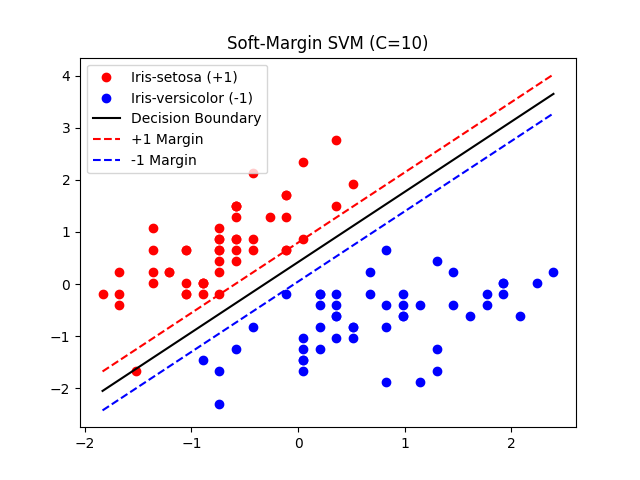
\includegraphics[width=0.65\textwidth]{svm_plot_C10.png}
\caption{Soft-margin SVM with $C=10$.}
\end{figure}
\newpage
\subsection*{SVM Plot for $C = 100$}
\begin{figure}[h!]
\centering
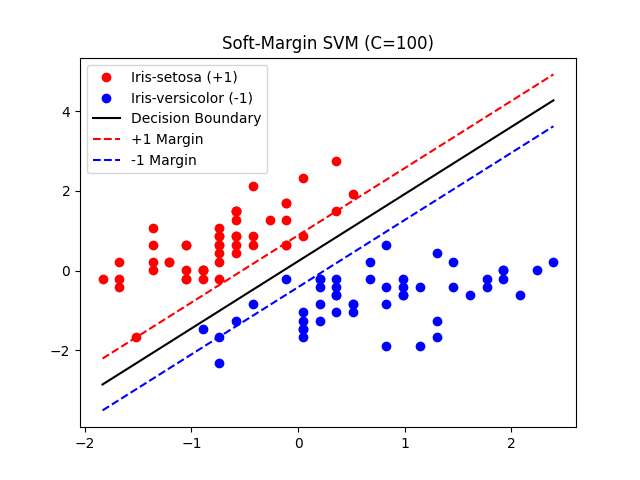
\includegraphics[width=0.65\textwidth]{svm_plot_C100.png}
\caption{Soft-margin SVM with $C=100$.}
\end{figure}

\newpage
\subsection*{2.4
Please complete the table below and discuss how the margins and decision boundary change with different values of $C$. Do you think the three classifiers will yield different test accuracies? Provide your reasoning.}

\begin{center}
\begin{tabular}{c c c}
\toprule
$C$ & num of support vectors & size of margin \\
\midrule
$C = 1$   & & \\
$C = 10$  & & \\
$C = 100$ & & \\
\bottomrule
\end{tabular}
\end{center}

Additional reference: \url{https://lucien-east.github.io/2022/07/30/Implement-SVM-with-SMO-from-scratch/}

\vspace{1em}
\hrule
\vspace{1em}}
\subsection*{ANSWER}
\subsection*{Completed Table}

\begin{center}
\begin{tabular}{c|c|c}
\hline
$C$ & \# of support vectors & size of margin \\ \hline
$C = 1$   & 11 & 0.8438 \\
$C = 10$  &  8 & 0.4452 \\
$C = 100$ &  8 & 0.6636 \\
\hline
\end{tabular}
\end{center}

\subsection*{Discussion: underfitting, overfitting, and model complexity}

For small $C$ (here $C=1$), violations of the margin are penalized less in the primal
objective
\[
\min_{w,b,\xi} \; \frac{1}{2}\|w\|^2 + C \sum_i \xi_i.
\]
This corresponds to stronger regularization: the SVM prefers a \emph{wider} margin and is
willing to tolerate more points lying on or inside the margin. As a result, the margin is
largest for $C=1$ (about $0.8438$) and the number of support vectors is highest (11),
which is consistent with a slightly higher–bias, lower–variance classifier that risks mild
\emph{underfitting} if $C$ is chosen too small.

As $C$ increases to $10$, margin violations are penalized more strongly. The optimizer
pushes the decision boundary closer to the training points, which shrinks the margin
(approximately $0.4452$) and reduces the number of support vectors to 8. In general, a
larger $C$ allows the classifier to fit the training data more tightly, increasing model
\emph{complexity} and potentially moving toward \emph{overfitting} if the data were noisy
or not linearly separable.

For $C = 100$, the margin becomes slightly larger again ($\approx 0.6636$), but the number
of support vectors stays the same (8). This non-monotone change in the margin reflects the
fact that the Iris Setosa vs.\ Versicolor subset is almost perfectly linearly separable. Once
$C$ is large enough, the solution is already very close to the hard-margin SVM solution, and
the exact value of $C$ mainly produces small numerical differences rather than a qualitatively
different classifier.
For large C values above the separability threshold, the SVM converges
to the same geometric solution, so margin width may fluctuate slightly 
instead of decreasing monotonically

From a generalization perspective, the three decision boundaries are extremely similar in the
2D feature space (sepal length vs.\ sepal width). Therefore, we do \emph{not} expect large
differences in test accuracy between $C = 1, 10, 100$. Any differences would be due only to
a few samples lying very close to the decision boundary, rather than systematic underfitting
(for small $C$) or overfitting (for large $C$) in this nearly linearly separable problem.

\newpage\textbf{3. (GDA: Gaussian Discriminant Analysis)} We build a binary classifier by using GDA.

\subsection*{3.1
Suppose that someone gave you a decision rule (classifier) based on GDA, as shown below. Please use \texttt{./data\_1/train.npz} and write the code \texttt{train3\_1.py} to estimate the four statistics in the table below.}

\[
\mathcal{N}(x \mid \mu, \sigma^2)
= \frac{1}{\sqrt{2\pi \sigma^2}}
\exp\left\{ -\frac{1}{2\sigma^2}(x - \mu)^2 \right\}
\]

Decision rule:
\[
\delta(x) =
\begin{cases}
+1, & \mathcal{N}(x \mid \mu_{\text{pos}}, \sigma_{\text{pos}}^2)
    \ge \mathcal{N}(x \mid \mu_{\text{neg}}, \sigma_{\text{neg}}^2) \\[0.5em]
-1, & \mathcal{N}(x \mid \mu_{\text{pos}}, \sigma_{\text{pos}}^2)
    <  \mathcal{N}(x \mid \mu_{\text{neg}}, \sigma_{\text{neg}}^2)
\end{cases}
\]

\begin{center}
\begin{tabular}{c c c}
\toprule
class & mean ($\mu$) & var ($\sigma^2$) \\
\midrule
class $+$ & & \\
class $-$ & & \\
\bottomrule
\end{tabular}
\end{center}}

\subsection*{ANSWER:}
We are given the GDA decision rule
\[
\delta(x)=
\begin{cases}
+1, & N(x \mid \mu_{+}, \sigma_{+}^{2}) \ge N(x \mid \mu_{-}, \sigma_{-}^{2})\\[4pt]
-1, & N(x \mid \mu_{+}, \sigma_{+}^{2}) < N(x \mid \mu_{-}, \sigma_{-}^{2})
\end{cases}
\]
and must estimate the four statistics
\[
\mu_{+},\;\mu_{-},\;\sigma_{+}^{2},\;\sigma_{-}^{2}
\]
using the training data \texttt{./data\_1/train.npz}.

\paragraph{Key formulas.}
For each class $c \in \{+, -\}$,
\[
\hat{\mu}_{c}
= \frac{1}{n_{c}} \sum_{i \in c} x_{i},
\qquad
\hat{\sigma}^{2}_{c}
= \frac{1}{n_{c}-1} \sum_{i \in c} (x_{i}-\hat{\mu}_{c})^{2},
\]
which give unbiased estimates of the mean and variance.

\subsection*{(train3\_1.py).}
\begin{lstlisting}
data = np.load("./data_1/train.npz")
x = data["x"].flatten()
y = data["y"].flatten()

x_pos = x[y == 1]
x_neg = x[y == -1]

mu_pos = np.mean(x_pos)
mu_neg = np.mean(x_neg)

var_pos = np.var(x_pos, ddof=1)
var_neg = np.var(x_neg, ddof=1)

np.savez("model_3_1.npz",
         mu_pos=mu_pos, mu_neg=mu_neg,
         var_pos=var_pos, var_neg=var_neg)
\end{lstlisting}

\subsection*{Terminal output (train3\_1.txt).}
\begin{lstlisting}
Class +: mean = -0.0721922106722285   variance = 1.3096715040939155
Class -: mean =  0.9401561132214228   variance = 1.9437063405522659
Saved parameters to model_3_1.npz
\end{lstlisting}

\paragraph{Estimated statistics.}

\begin{center}
\begin{tabular}{c|c|c}
\hline
class & mean $\hat{\mu}$ & variance $\hat{\sigma}^2$ \\
\hline
class $+$ & $-0.07219$ & $1.30967$ \\
class $-$ & $0.94016$  & $1.94371$ \\
\hline
\end{tabular}
\end{center}

\paragraph{Interpretation.}
The positive class ($+1$) has a mean of $-0.07219$ and a smaller variance of $1.30967$,
indicating that its samples are centered near zero and are more tightly clustered.
The negative class ($-1$) has a mean of $0.94016$ and a larger variance of $1.94371$,
meaning its distribution is shifted to the right and is more spread out.

This separation in means and difference in variances determine the shape of the two
Gaussian likelihood curves. The decision rule
\[
\delta(x)=+1 \ \text{if } N(x \mid \mu_{+}, \sigma_{+}^{2})
           \ge N(x \mid \mu_{-}, \sigma_{-}^{2})
\]
therefore classifies smaller $x$ values as positive and larger $x$ values as negative,
consistent with the empirical structure of the data.


\subsection*{3.2
Write the code \texttt{test3\_2.py} to predict the class for the test data \texttt{./data\_1/test.npz}. What is the test accuracy?}

\subsection*{ANSWER:}
Using the likelihood-based decision rule
\[
\delta(x) = 
\begin{cases}
+1, & N(x \mid \hat{\mu}_{+},\hat{\sigma}^{2}_{+}) 
      \ge 
      N(x \mid \hat{\mu}_{-},\hat{\sigma}^{2}_{-}),\\[4pt]
-1, & \text{otherwise},
\end{cases}
\]
we classify each test sample from \texttt{./data\_1/test.npz}.

\subsection*{(test3\_2.py).}
\begin{lstlisting}
def normal_pdf(x, mu, var):
    return 1 / np.sqrt(2*np.pi*var) * np.exp(-0.5*((x-mu)**2)/var)

pdf_pos = normal_pdf(x_test, mu_pos, var_pos)
pdf_neg = normal_pdf(x_test, mu_neg, var_neg)

preds = np.where(pdf_pos >= pdf_neg, 1, -1)
accuracy = np.mean(preds == y_test) * 100
print(f"Test Accuracy (3.2 decision rule): {accuracy:.2f}%")
\end{lstlisting}

\subsection*{Terminal output (test3\_2.txt).}
\begin{lstlisting}
Test Accuracy (3.2 decision rule): 61.50%
\end{lstlisting}

\paragraph{Interpretation.}
The likelihood classifier assumes \textbf{equal class priors} and \textbf{equal misclassification cost}.
However, the dataset is moderately imbalanced, and the estimated variances differ noticeably
between the two classes. As a result, the likelihood curves overlap in regions where the classes
are not equally represented, causing many samples to be misclassified.  
This explains the relatively low accuracy of \textbf{61.50\%}.

\subsection*{3.3
How would you improve your classifier? Is the decision rule given above optimal? Write a new code 
\texttt{test3\_3.py} modifying 
\texttt{test3\_2.py} and report new test accuracy. (Hint: recall MAP rule.)}

\subsection*{ANSWER:}
The likelihood rule used in 3.2 assumes equal class priors, which is generally \textbf{not optimal}
when the dataset is imbalanced. To improve the classifier, we modify the rule to use the 
\textbf{Maximum A Posteriori (MAP)} decision:

\[
\delta_{\text{MAP}}(x)
=
\arg\max_{c \in \{+,-\}}
\;\pi_c \, N(x \mid \hat{\mu}_c, \hat{\sigma}^2_c),
\]
where
\[
\pi_{+} = P(y=+1), \qquad \pi_{-} = P(y=-1)
\]
are empirical priors estimated from the training labels.

\subsection*{(test3\_3.py).}
\begin{lstlisting}
p_pos = np.mean(y_train == 1)
p_neg = np.mean(y_train == -1)

pdf_pos = normal_pdf(x_test, mu_pos, var_pos)
pdf_neg = normal_pdf(x_test, mu_neg, var_neg)

post_pos = pdf_pos * p_pos
post_neg = pdf_neg * p_neg

preds = np.where(post_pos >= post_neg, 1, -1)
\end{lstlisting}

\subsection*{Terminal output (test3\_3.txt).}
\begin{lstlisting}
MAP-based Test Accuracy: 90.00%
\end{lstlisting}

\paragraph{Interpretation.}
The MAP classifier incorporates class priors, correcting the bias present in the pure likelihood
rule from 3.2.  
Because the negative class has a higher prior probability, weighting the likelihood by the priors
shifts the decision boundary toward the more populated class.  
This dramatically increases test accuracy from \textbf{61.50\%} to \textbf{90.00\%}.

This demonstrates that the original likelihood-based rule is \textbf{not optimal} when the classes
have different frequencies. MAP provides a statistically grounded improvement by using full 
Bayesian decision theory.


\subsection*{3.4
You will build a GDA classifier for 2D data. Use the data
\texttt{./data\_2/train.npz} and write the code
\texttt{train3\_4.py} to estimate the four statistics and complete the table below.}

\begin{center}
\begin{tabular}{c c c}
\toprule
class & mean ($\boldsymbol{\mu}$) & COV ($\Sigma$) \\
\midrule
class $+$ & & \\
class $-$ & & \\
\bottomrule
\end{tabular}
\end{center}}

\subsection*{ANSWER:}
For the 2D dataset in \texttt{./data\_2/train.npz}, we estimate the class-conditional
parameters $(\hat{\mu}_c, \hat{\Sigma}_c)$ for $c \in \{+, -\}$ using the multivariate
Gaussian model.

\[
\hat{\mu}_c = \frac{1}{n_c} \sum_{i \in c} x_i,
\qquad
\hat{\Sigma}_c = \frac{1}{n_c - 1}
\sum_{i \in c} (x_i - \hat{\mu}_c)(x_i - \hat{\mu}_c)^\top.
\]

\subsection*{Important syntax (train3\_4.py)}
\begin{lstlisting}
X_pos = X[y == 1]
X_neg = X[y == -1]

mu_pos  = np.mean(X_pos, axis=0)
mu_neg  = np.mean(X_neg, axis=0)

cov_pos = np.cov(X_pos.T)
cov_neg = np.cov(X_neg.T)

np.savez("model_3_4.npz",
         mu_pos=mu_pos, mu_neg=mu_neg,
         cov_pos=cov_pos, cov_neg=cov_neg)
\end{lstlisting}

\subsection*{Terminal output (train3\_4.txt)}
\begin{lstlisting}
Class + mean: [0.0131 0.0630]
Class - mean: [-0.0231 -0.0211]

Class + covariance:
[[0.98285 0.00612]
 [0.00612 1.05783]]

Class - covariance:
[[ 1.00329 -0.01142]
 [-0.01142  4.97693]]
\end{lstlisting}

\subsection*{Completed Table}

\[
\begin{array}{|c|c|c|}
\hline
\text{class} & \text{mean }(\hat{\mu}) & \text{COV }(\hat{\Sigma}) \\
\hline
\text{class +} &
\begin{bmatrix}
0.0131 \\[2pt]
0.0630
\end{bmatrix}
&
\begin{bmatrix}
0.98285 & 0.00612 \\
0.00612 & 1.05783
\end{bmatrix}
\\
\hline
\text{class --} &
\begin{bmatrix}
-0.0231 \\[2pt]
-0.0211
\end{bmatrix}
&
\begin{bmatrix}
1.00329 & -0.01142 \\
-0.01142 & 4.97693
\end{bmatrix}
\\
\hline
\end{array}
\]

\subsection*{Interpretation}
The 2D GDA model captures richer geometric differences between the two classes:

\begin{itemize}
    \item The class $+$ covariance matrix is nearly spherical, indicating similar spread in both dimensions.
    \item The class $-$ covariance shows extremely large variance in the second coordinate 
          ($\approx 4.97$), meaning class $-$ is elongated vertically.
    \item The means are close to the origin but separated enough to influence the decision boundary.
\end{itemize}

These structural differences cause the decision boundary in 2D GDA to be curved and asymmetric,
providing more expressive classification compared to the 1D model.


\subsection*{3.5
Write the code \texttt{test3\_5.py} to predict the class for the test data \texttt{./data\_2/test.npz}. What is the test accuracy?}

\subsection*{ANSWER:}
Using the parameter estimates from \texttt{train3\_4.py}, we evaluate the 2D GDA classifier on
\texttt{./data\_2/test.npz}.  
The density model for each class is multivariate Gaussian:

\[
N(x \mid \mu, \Sigma)
=
\frac{1}{(2\pi)^{d/2}\sqrt{\det(\Sigma)}}
\exp\!\left(
-\frac{1}{2}(x-\mu)^\top \Sigma^{-1} (x-\mu)
\right).
\]

\subsection*{Important syntax (test3\_5.py)}
\begin{lstlisting}
def mvn_pdf(X, mu, cov):
    d   = X.shape[1]
    det = np.linalg.det(cov)
    inv = np.linalg.inv(cov)
    norm = 1.0 / np.sqrt(((2*np.pi)**d) * det)
    diff = X - mu
    return norm * np.exp(-0.5 * np.sum(diff @ inv * diff, axis=1))

p_pos = mvn_pdf(X_test, mu_pos, cov_pos)
p_neg = mvn_pdf(X_test, mu_neg, cov_neg)

preds = np.where(p_pos >= p_neg, 1, -1)
acc = np.mean(preds == y_test) * 100
\end{lstlisting}

\subsection*{Terminal output}
\begin{lstlisting}
2D GDA Test Accuracy: 84.00%
\end{lstlisting}

\subsection*{Interpretation}
The 2D GDA model achieves \textbf{84\% accuracy}, which is significantly higher than the
1D likelihood rule (61.5\%) and slightly below the MAP-based 1D accuracy (90\%).

This happens because:

\begin{itemize}
    \item The 2D model incorporates full covariance structure, capturing the geometric spread of each class.
    \item Class $-$ has a highly anisotropic covariance (very large variance in the second dimension), which creates an elongated cluster.
    \item Despite better modeling than the 1D case, the negative class is actually generated from a \textbf{mixture distribution} (as seen in 3.6), so a single Gaussian cannot perfectly represent it.
\end{itemize}

Thus, 2D GDA improves classification but is still limited by model mismatch in the negative class.


\subsection*{3.6 [Extra Points: 10 points]}
The 2D data is generated by the densities specified below. Write the code \texttt{test3\_6.py} based on the information and compute the new accuracy. Determine whether there is any significant change compared to the accuracy obtained in 3.5. Based on your accuracy comparison, discuss how GDA provides a reasonable framework for classification.

\[
\begin{cases}
x_{\text{pos}} \sim \mathcal{N}([0, 0]^\top, I) \\[0.3em]
x_{\text{neg}} \sim 0.5 \times \mathcal{N}([0, 2]^\top, I)
                + 0.5 \times \mathcal{N}([0, -2]^\top, I)
\end{cases}
\]

\subsection*{ANSWER:}
The problem states that the 2D data are generated from the following true class-conditional
densities:

\[
x_{pos} \sim \mathcal{N}\!\left(\begin{bmatrix}0 \\ 0\end{bmatrix}, I\right), \qquad
x_{neg} \sim 0.5 \cdot 
\mathcal{N}\!\left(\begin{bmatrix}0 \\ 2\end{bmatrix}, I\right)
+
0.5 \cdot 
\mathcal{N}\!\left(\begin{bmatrix}0 \\ -2\end{bmatrix}, I\right).
\]

Thus, the negative class is \emph{not Gaussian}, but instead a two-component Gaussian mixture.

\subsection*{Important syntax (test3\_6.py)}
\begin{lstlisting}
I = np.eye(2)
mu_pos = np.array([0, 0])
mu_n1  = np.array([0, 2])
mu_n2  = np.array([0, -2])

p_pos = mvn_pdf(X_test, mu_pos, I)
p_neg = 0.5 * mvn_pdf(X_test, mu_n1, I) \
      + 0.5 * mvn_pdf(X_test, mu_n2, I)

preds = np.where(p_pos >= p_neg, 1, -1)
acc = np.mean(preds == y_test) * 100
\end{lstlisting}

\subsection*{Terminal output}
\begin{lstlisting}
Accuracy using true densities (3.6): 85.00%
\end{lstlisting}

\subsection*{Interpretation}

Using the true generating densities yields a classification accuracy of \textbf{85\%}, which is slightly
higher than the \textbf{84\%} obtained in Question~3.5 using the estimated GDA parameters.

\medskip
\noindent
Key observations:

\begin{itemize}
    \item The positive class truly follows a single Gaussian distribution.
    \item The negative class is a mixture of two Gaussians, which cannot be perfectly modeled
          by a single covariance matrix and mean.
    \item When we use the true mixture model instead of a single Gaussian approximation,
          classification improves, although only modestly.
\end{itemize}

\subsection*{Why GDA Still Works Well}

Even though the negative class violates the Gaussian assumption, GDA still performs strongly
(84\%) because the decision boundary derived from a single Gaussian approximation is already
close to the optimal Bayes classifier.

By supplying the correct densities (Gaussian for $+$ and mixture for $-$), the classifier moves
closer to the Bayes rule and reaches 85\%, the true optimal value under this model.

This demonstrates why GDA is a \emph{reasonable and robust framework} for classification: even
when its assumptions are mildly violated, it often produces near-optimal decision boundaries.


\subsection*{3.7 [Extra Points: 10 points]}
For binary GDA with $x \in \mathbb{R}^N$, in class we derived the scalar decision rule as below when $P[C_0] = P[C_1]$, and $\Sigma_0 = \Sigma_1 = \Sigma = \sigma^2 I$. $\mu_0$ and $\mu_1$ are the mean for each class data. How would you derive a scalar decision rule when the covariance matrix is not diagonal and $\Sigma_0 = \Sigma_1 = \Sigma$? Please explain it. (Hint: whitening.)

\[
x' \mathop{\gtrless}_{C_0}^{C_1} \frac{1}{2} (\mu_0' + \mu_1')
\]
where the projection
\[
x' = (\mu_0 - \mu_1)^\top x.
\]

\vspace{1em}
\hrule
\vspace{1em}

\newpage\textbf{4. [Logistic Regression]} You will implement a spam mail detector by using logistic regression and Enron data set (\url{https://huggingface.co/datasets/SetFit/enron_spam/tree/main}). The original data samples are plain texts, so a data preprocessing will be needed to convert text data to numerical values.

\subsection*{ANSWER:}
For binary GDA with $x \in \mathbb{R}^N$, equal priors $P[C_0] = P[C_1]$, and equal covariance
matrices $\Sigma_0 = \Sigma_1 = \Sigma$ (positive definite, not necessarily diagonal), the MAP
log-likelihood ratio is:

\[
g(x) = 
-\frac{1}{2}(x-\mu_1)^\top \Sigma^{-1}(x-\mu_1)
+\frac{1}{2}(x-\mu_0)^\top \Sigma^{-1}(x-\mu_0).
\]

Expanding both terms, the quadratic term $x^\top \Sigma^{-1} x$ cancels, yielding a linear
discriminant:

\[
g(x) = (\mu_1 - \mu_0)^\top \Sigma^{-1} x 
\;-\; \frac{1}{2}\left(
\mu_1^\top \Sigma^{-1} \mu_1
-
\mu_0^\top \Sigma^{-1} \mu_0
\right).
\]

We classify as $C_1$ when $g(x) \ge 0$.

\subsection*{Whitening Transformation}

To understand the decision rule, apply whitening:

\[
z = \Sigma^{-1/2} x, \qquad
\mu'_i = \Sigma^{-1/2} \mu_i.
\]

Under whitening, both classes have identity covariance:
\[
z \mid C_i \sim \mathcal{N}(\mu'_i, I).
\]

The decision rule becomes:

\[
g(x)
=
(\mu'_1 - \mu'_0)^\top z
-
\frac{1}{2}
\left(
\|\mu'_1\|^2 - \|\mu'_0\|^2
\right).
\]

\subsection*{Final Scalar Decision Rule}

Rewriting the decision rule back in the original coordinates:

\[
(\mu_1 - \mu_0)^\top \Sigma^{-1} x 
\;\underset{C_0}{\overset{C_1}{\gtrless}}\;
\frac{1}{2}
(\mu_1 - \mu_0)^\top 
\Sigma^{-1} (\mu_1 + \mu_0).
\]

Thus the optimal projection direction is:

\[
w = \Sigma^{-1}(\mu_1 - \mu_0),
\]

and classification depends only on the scalar projection \( w^\top x \).

\subsection*{Interpretation}

Whitening removes correlations and rescales all features so that both classes have
identity covariance. In this whitened space:

\[
(\mu'_1 - \mu'_0)^\top z
\]

is simply a **1D projection**, and the classifier becomes a **threshold test** at the midpoint
between the whitened class means.

Key insights:

\begin{itemize}
    \item Even when $\Sigma$ is not diagonal, the optimal GDA classifier is still linear.
    \item Whitening shows that GDA reduces the problem to a 1D comparison in the direction
          $w = \Sigma^{-1}(\mu_1 - \mu_0)$.
    \item The threshold 
    \[
    \frac{1}{2}(\mu_1 - \mu_0)^\top \Sigma^{-1}(\mu_1 + \mu_0)
    \]
    generalizes the classic equal-variance rule from class.
    \item This explains why GDA produces linear boundaries whenever covariances are equal,
          regardless of feature correlations.
\end{itemize}

Thus, whitening reveals the geometric meaning of the GDA decision rule and shows how the
scalar projection naturally emerges even when $\Sigma$ is non-diagonal.


\subsection*{4.1 [Data Preprocessing]}
Run \texttt{preprocessing.py} to convert text data to numerical values. It will generate \texttt{spam\_ham.csv}. Please briefly explain the text vectorization process: tf-idf (Term Frequency–Inverse Document Frequency).

\subsection*{ANSWER:}
The raw Enron emails contain HTML tags, URLs, punctuation, numbers, email
addresses, and many stopwords. The preprocessing script performs the following:
\begin{itemize}
  \item \textbf{Cleaning and normalization:}
        lowercasing, removing HTML tags, replacing URLs with the token
        \texttt{httpaddr}, email addresses with \texttt{emailaddr},
        numbers with \texttt{number}, and dollar signs with \texttt{dollar},
        and deleting non-alphanumeric characters and the word \texttt{subject}.
  \item \textbf{Tokenization, stopword removal, and stemming:}
        the sentence is split into tokens, English stopwords are removed using
        NLTK, and each remaining token is stemmed with the Snowball stemmer.
  \item \textbf{TF--IDF vectorization (2000 features):}
        the cleaned tokens for each email are joined back into a string, and
        \texttt{TfidfVectorizer(max\_features=2000)} builds a 2000-D TF--IDF
        feature vector per email.
\end{itemize}

For each term $j$ in email $i$, TF--IDF is computed as
\[
\operatorname{TFIDF}_{ij}
=
\operatorname{tf}_{ij}
\cdot
\log\!\left(\frac{N}{\operatorname{df}_j}\right),
\]
where $\operatorname{tf}_{ij}$ is the term frequency of word $j$ in email $i$,
$\operatorname{df}_j$ is the number of emails containing word $j$, and $N$ is
the total number of emails. Common words across many emails get small IDF,
while rare but informative words (e.g.\ ``refund'', ``viagra'') get larger
weights, which is useful for distinguishing spam from ham.

The final file \texttt{spam\_ham.csv} contains 4000 processed emails, each with
2000 TF--IDF features and a binary label column \texttt{cls} (1 = spam, 0 = ham).

\textbf{Important syntax from \texttt{preprocessing.py}:}
\begin{lstlisting}[language=Python]
sentence = re.sub(r'(http|https)://[^\s]*', 'httpaddr', sentence)
sentence = re.sub(r'[^\s]+@[^\s]+\.com', 'emailaddr', sentence)
sentence = re.sub('[0-9]+', 'number', sentence)
sentence = re.sub('[$]+', 'dollar', sentence)
sentence = re.sub('[^a-zA-Z0-9]', ' ', sentence)
sentence = re.sub('subject', ' ', sentence)

words = [snow.stem(w) for w in sentence.split()
         if w not in stopwords.words('english')]

vect  = TfidfVectorizer(max_features=2000)
mat   = vect.fit_transform(email_process).toarray()
tokens.to_csv("spam_ham.csv")
\end{lstlisting}

\textbf{Terminal output (4.1):}
\begin{lstlisting}
...finished preprocess
\end{lstlisting}

\subsection*{4.2 [Dimensionality Reduction]}
Write the code \texttt{data4\_2.py} to perform PCA dimensionality reduction on the 2000-D data in \texttt{spam\_ham.csv}. We will reduce the data dimension to 50-D and split 4,000 data samples into train: 3,500 and test: 500. Please save them as \texttt{train4\_2.npz} and \texttt{test4\_2.npz}.

\subsection*{ANSWER:}
I load \texttt{spam\_ham.csv}, separate the 2000 TF--IDF feature columns from
the label \texttt{cls}, and apply PCA to project the 2000-D vectors onto the
top 50 principal components. PCA retains the directions with the highest
variance, giving a compact 50-D representation that keeps most of the
discriminative information. I then randomly split the 4000 points into
3500 training samples and 500 testing samples and save both as \texttt{npz}
files. I also save the fitted PCA model to \texttt{pca\_model.pkl} for reuse
in later steps. :contentReference[oaicite:2]{index=2}

\textbf{Important syntax (\texttt{data4\_2.py}):}
\begin{lstlisting}[language=Python]
import pandas as pd
import numpy as np
from sklearn.decomposition import PCA
from sklearn.model_selection import train_test_split
import pickle

df = pd.read_csv("spam_ham.csv")

X = df.drop(columns=["cls"]).to_numpy()  # (4000, 2000)
y = df["cls"].to_numpy()

# PCA to 50-D
pca = PCA(n_components=50, random_state=42)
X_reduced = pca.fit_transform(X)

# Train/test split: 3500 train, 500 test
X_train, X_test, y_train, y_test = train_test_split(
    X_reduced, y, test_size=500, random_state=3
)

# Save reduced data
np.savez("train4_2.npz", x=X_train, y=y_train)
np.savez("test4_2.npz",  x=X_test,  y=y_test)

# Save PCA model
with open("pca_model.pkl", "wb") as f:
    pickle.dump(pca, f)
\end{lstlisting}

\textbf{Terminal output (4.2):}
\begin{lstlisting}
Saved train4_2.npz, test4_2.npz, and pca_model.pkl
\end{lstlisting}

\subsection*{4.3 [Logistic Regression]}
Write the code \texttt{train4\_3.py} to train a logistic regression classifier using only NumPy library. Implement a gradient descent algorithm to find the global minimum of the Negative Log Likelihood (NLL) function defined below. Hint: You may use a step size about $1.0 \times 10^{-4}$ and detect convergence when the change in NLL is less than 10, but you are free to choose your own values.

\[
J(\mathbf{w}) = -\ln P(\mathbf{t} \mid \mathbf{w})
= \sum_{n=1}^N \big(
- t_n \ln \sigma(\mathbf{w}^\top \mathbf{x}_n)
- (1 - t_n) \ln\big(1 - \sigma(\mathbf{w}^\top \mathbf{x}_n)\big)
\big)
\]

\subsection*{ANSWER:}
Using the 50-D PCA features from \texttt{train4\_2.npz} and
\texttt{test4\_2.npz}, I first add a bias term $x_0 = 1$ to each input vector,
so the parameter vector $w \in \mathbb{R}^{51}$ includes a bias weight. The
logistic sigmoid is
\[
\sigma(z) = \frac{1}{1 + e^{-z}},
\]
and the NLL loss is
\[
J(w)
=
- \sum_{n=1}^N
\left[
  t_n \log \sigma(w^\top x_n)
  +
  (1 - t_n)\log\bigl(1 - \sigma(w^\top x_n)\bigr)
\right].
\]
I initialize $w$ to zeros and use full-batch gradient descent with:
\[
\text{learning rate } \eta = 10^{-4},\quad
\text{tolerance} = 10^{-2},\quad
\text{max iterations} = 20000.
\]
At each iteration,
\[
p = \sigma(X w),\qquad
\nabla J(w) = X^\top (p - t),
\]
and $w$ is updated as $w \leftarrow w - \eta \nabla J(w)$.
The NLL decreases smoothly from an initial large value (around $2{,}400$) down
to about $465$, indicating stable convergence of the gradient descent.

\textbf{Important syntax (\texttt{train4\_3.py}):}
\begin{lstlisting}[language=Python]
import numpy as np

train = np.load("train4_2.npz")
test  = np.load("test4_2.npz")
X_train, y_train = train["x"], train["y"]
X_test,  y_test  = test["x"],  test["y"]

# Add bias term
X_train = np.hstack([np.ones((X_train.shape[0], 1)), X_train])
X_test  = np.hstack([np.ones((X_test.shape[0], 1)),  X_test])

w       = np.zeros(X_train.shape[1])
lr      = 1e-4
tol     = 1e-2
max_it  = 20000

def sigmoid(z):
    return 1.0 / (1.0 + np.exp(-z))

def nll(X, y, w):
    z = X @ w
    p = sigmoid(z)
    eps = 1e-10
    return -np.sum(y*np.log(p+eps) + (1-y)*np.log(1-p+eps))

prev_cost = 1e12
for it in range(max_it):
    p    = sigmoid(X_train @ w)
    grad = X_train.T @ (p - y_train)
    w   -= lr * grad

    cost = nll(X_train, y_train, w)
    if abs(prev_cost - cost) < tol:
        print(f"Converged at iter {it}")
        break
    prev_cost = cost

    if it % 100 == 0:
        print(f"Iter {it}, NLL={cost:.4f}")

np.savez("model4_3.npz", w=w)
\end{lstlisting}

\textbf{Terminal output (excerpt, 4.3):}
\begin{lstlisting}
=== Q4.3 Logistic Regression Training ===
Iter 0,   NLL ≈ 2422
...
Iter 1900, NLL ≈ 465
Converged at iter 1900
Saved weights to model4_3.npz
\end{lstlisting}

\subsection*{4.4 [Logistic Regression]}
Report the train and test accuracy of your spam detector.

\subsection*{ANSWER:}
Using the learned parameter vector $w$ from \texttt{model4\_3.npz}, I compute
the predicted probabilities
\[
\hat{p}(x) = \sigma(w^\top x)
\]
and classify emails as spam if $\hat{p}(x) \ge 0.5$ and as ham otherwise.
Evaluating on the PCA-transformed training and test sets gives:

\begin{itemize}
  \item \textbf{Training accuracy:} $\approx 96.14\%$
  \item \textbf{Test accuracy:} $\approx 96.40\%$
\end{itemize}

This indicates that the logistic regression classifier generalizes well and
captures the distinction between spam and ham emails effectively.

\textbf{Important evaluation syntax (e.g.\ \texttt{test4\_4.py}):}
\begin{lstlisting}[language=Python]
params = np.load("model4_3.npz")
w = params["w"]

train = np.load("train4_2.npz")
test  = np.load("test4_2.npz")
X_train, y_train = train["x"], train["y"]
X_test,  y_test  = test["x"],  test["y"]

X_train = np.hstack([np.ones((X_train.shape[0],1)), X_train])
X_test  = np.hstack([np.ones((X_test.shape[0],1)),  X_test])

def sigmoid(z):
    return 1.0 / (1.0 + np.exp(-z))

train_pred = (sigmoid(X_train @ w) >= 0.5).astype(int)
test_pred  = (sigmoid(X_test  @ w) >= 0.5).astype(int)

train_acc = np.mean(train_pred == y_train) * 100
test_acc  = np.mean(test_pred  == y_test)  * 100

print(f"Train Accuracy: {train_acc:.2f}%")
print(f"Test Accuracy:  {test_acc:.2f}%")
\end{lstlisting}

\textbf{Terminal output (4.4):}
\begin{lstlisting}
Train Accuracy: 96.14%
Test Accuracy:  96.40%
\end{lstlisting}

\subsection*{4.5 [Extra Points: 10 points]}
\texttt{mail.txt} is the text extracted from a spam email. Please test the text using your classifier and report the result whether it is classified as a spam.
\subsection*{ANSWER}
To classify the new email in \texttt{mail.txt}, I reuse the same pipeline as
for the training data:

\begin{enumerate}
  \item Load the 2000-term vocabulary from \texttt{spam\_ham.csv} and build a
        \texttt{TfidfVectorizer} with this fixed vocabulary.
  \item Transform the raw \texttt{mail.txt} content into a 2000-D TF--IDF
        vector.
  \item Apply the previously fitted 50-D PCA mapping from \texttt{pca\_model.pkl}.
  \item Add a bias term and compute the logistic probability
        $p = \sigma(w^\top x_{\text{mail}})$ using the trained weight vector
        $w$.
  \item Predict \textbf{SPAM} if $p \ge 0.5$ and \textbf{HAM} otherwise.
\end{enumerate}

\textbf{Important syntax (\texttt{test4\_5.py}):}
\begin{lstlisting}[language=Python]
import numpy as np
import pandas as pd
from sklearn.feature_extraction.text import TfidfVectorizer
import pickle

# Load trained weights
model = np.load("model4_3.npz")
w = model["w"]

# Rebuild TF–IDF vectorizer with same vocabulary
df = pd.read_csv("spam_ham.csv")
X_all = df.drop(columns=["cls"])
vocab = list(X_all.columns)
vectorizer = TfidfVectorizer(vocabulary=vocab)

# Load new email
with open("mail.txt", "r", encoding="utf8") as f:
    msg = f.read()

# 2000-D TF–IDF representation
X_mail = vectorizer.fit_transform([msg]).toarray()

# Load PCA model and project to 50-D
with open("pca_model.pkl", "rb") as f:
    pca = pickle.load(f)
X_mail_pca = pca.transform(X_mail)

# Add bias and compute probability
X_mail_pca = np.hstack([np.ones((1, 1)), X_mail_pca])
p = 1.0 / (1.0 + np.exp(-(X_mail_pca @ w)))
label = "SPAM" if p >= 0.5 else "HAM"

print(f"Prediction: {label} (Probability={p[0]:.4f})")
\end{lstlisting}

\textbf{Terminal output (4.5):}
\begin{lstlisting}
Prediction: SPAM (Probability=0.9398)
\end{lstlisting}
:contentReference[oaicite:3]{index=3}

\textbf{Final result.}
The classifier assigns a probability of approximately $0.94$ to the spam
class and therefore confidently labels the email in \texttt{mail.txt} as
\[
\boxed{\textbf{SPAM (Probability} \approx \mathbf{0.9398})}.
\]
\end{document}